\documentclass[12pt]{article}

%Packages%
\usepackage{graphicx, parskip}
\usepackage[export]{adjustbox}

%Meta%
\title{Distributed Database Systems - Introduction}
\author{Diego ROJAS}

%Document%
\begin{document}

\maketitle

\section{Distributed data processing}

A \textit{distributed computing system} consists in a number of autonomous programs interconnected by a computer network.

\textit{Processing logic}, \textit{control}, \textit{function} and \textit{data} can all be distributed within a system.

\section{What is a Distributed Database System?}

A \textit{Distributed Database System} (DDBS) can be defined as a collection of multiple, logically interrelated databases distributed over a computer network.

A \textit{Distributed Database Management System} (DDBMS) is defined as the software system that permits the management of the distributed database and makes the distribution transparent to the users

\section{Data Delivery Alternatives}

In a DDBS, data delivery consists in three things.

\begin{itemize}
	\item The \textit{delivery mode} (\textit{push only}, \textit{pull only}, \textit{hybrid})
	\item The \textit{frequency} (\textit{periodic}, \textit{conditional}, \textit{ad-hoc/irregular})
	\item The \textit{communication method} (\textit{unicast}, \textit{one-to-many})
\end{itemize}

\section{Promises of DDBSs}

\subsection{Transparent Management of Distributed and Replicated Data}

DDBSs are \textit{transparent} meaning the implementation details are hidden from the end-user.

DDBS may enforce:
\begin{itemize}
	\item \textit{Data independence} whereby the \textit{logical representation} (schema definition) is decoupled from the \textit{physical representation} (on-disk storage).
	\item \textit{Location transparency} whereby the storage location is hidden.
	\item \textit{Network transparency} whereby the network implementation is hidden.
	\item \textit{Naming transparency} whereby the names are unique.
	\item \textit{Replication transparency} whereby replication (or lack thereof) is hidden.
	\item \textit{Fragmentation transparency} whereby possibly fragmented data behaves as if whole.	
\end{itemize}
Full transparency may hurt performance, data management, modularity and more. Query languages, operating systems and DDBMSs may provide different levels of transparency to manage the tradeoff between ease-of-use and performance.

\subsection{Reliability through distributed transactions}

DDBSs prevent SPoF. The failure of a single site, or the failure of a communication link which makes one or more sites unreachable, is not sufficient to bring down the entire system.

DDBSs implement transactions which guarantees \textit{data consistency}.

\subsection{Improved Performance}

\textit{Data localization} whereby data is stored next to its point of use, increases the performance of a DDBS.

Contention for I/O and CPU is limited compared to centralised databases.

\subsection{Easier System Expansion}

Increase in database size can be addressed by allocating additional
 nodes to a distributed database cluster.

While mainframes are still very useful, a collection of small machines is sometimes more economically viable. 

\section{Complications Introduced by Distribution}

\begin{itemize}
	\item Data replication implies keeping the data consistent when it's updated.
	\item Failure of a component must not break data consistency.
	\item Synchronisation of operations is considerably harder than for a centralised system.
\end{itemize}

\section{Design Issues}

\subsection{Distributed Database Design}

Within a DDBS, data can be:
\begin{itemize}
	\item \textit{Replicated} where the entire database is stored in each node. Databases can also be \textit{partially replicated}.
	\item \textit{Partitioned} (or \textit{non-replicated}) where each node contains a disjoint subset of the data.
\end{itemize}

\textit{Fragmentation} refers to the separation of the database into partitions called \textit{fragments}.

\textit{Distribution} is the optimum distribution of fragments.

Fragmentation and distribution aim at lowering cost of storage, communication overhead and processing of transactions. This problem is NP-hard therefore it is usually solved using heuristics.

\subsection{Distributed Directory Management}

Must define if and how directories are fragmented across a DDBS.

\subsection{Distributed Query Processing}

Must define when and how to distribute queries to maximize performance.

\subsection{Distributed Concurrency Control}

One of the most researched issues introduced by DDBSs.

DDBSs must ensure that all the values of multiple copies of every data item converge to the same value. This is called \textit{mutual consistency}.

\subsection{Distributed Deadlock Management}

Must define how locking is used to avoid deadlocks.

\subsection{Reliability of Distributed DBMS}

Must ensure failure of a location or communication failure between two locations is accounted for and doesn't bring the system down.

\subsection{Replication}

If the database is replicated, the consistency of replicas becomes an issue. Replication can either be \textit{lazy} whereby a transaction completes before the result of the transaction is propagated to all the sites or \textit{eager} whereby all updates must be propagated before the transaction returns.

\subsection{Relationship among Problems}

The aforementioned problems are closely related. For example, concurrency control is linked to deadlock management. The solution to one problem can affect the solution to another.

\section{Distributed DBMS Architecture}

There are three majors DDBS architectures.
\begin{itemize}
	\item Client/server systems
	\item Peer-to-peer distributed DBMS
	\item Multidatabase systems
\end{itemize}

\subsection{ANSI/SPARC Architecture}

The ANSI/SPARC architecture defines three views of a database:
\begin{itemize}
	\item \textit{External view} which is that of the end user.
	\item \textit{Conceptual view} which is that of the database.
	\item \textit{Internal view} which is that of the entreprise.
\end{itemize}

This provides the basis for data independence as one view can change without affecting the others. The separation of the external schemas from the conceptual schema enables \textit{logical data independence}, while the separation of the conceptual schema from the internal schema allows \textit{physical data independence}.

\subsection{A Generic Centralized DBMS Architecture}

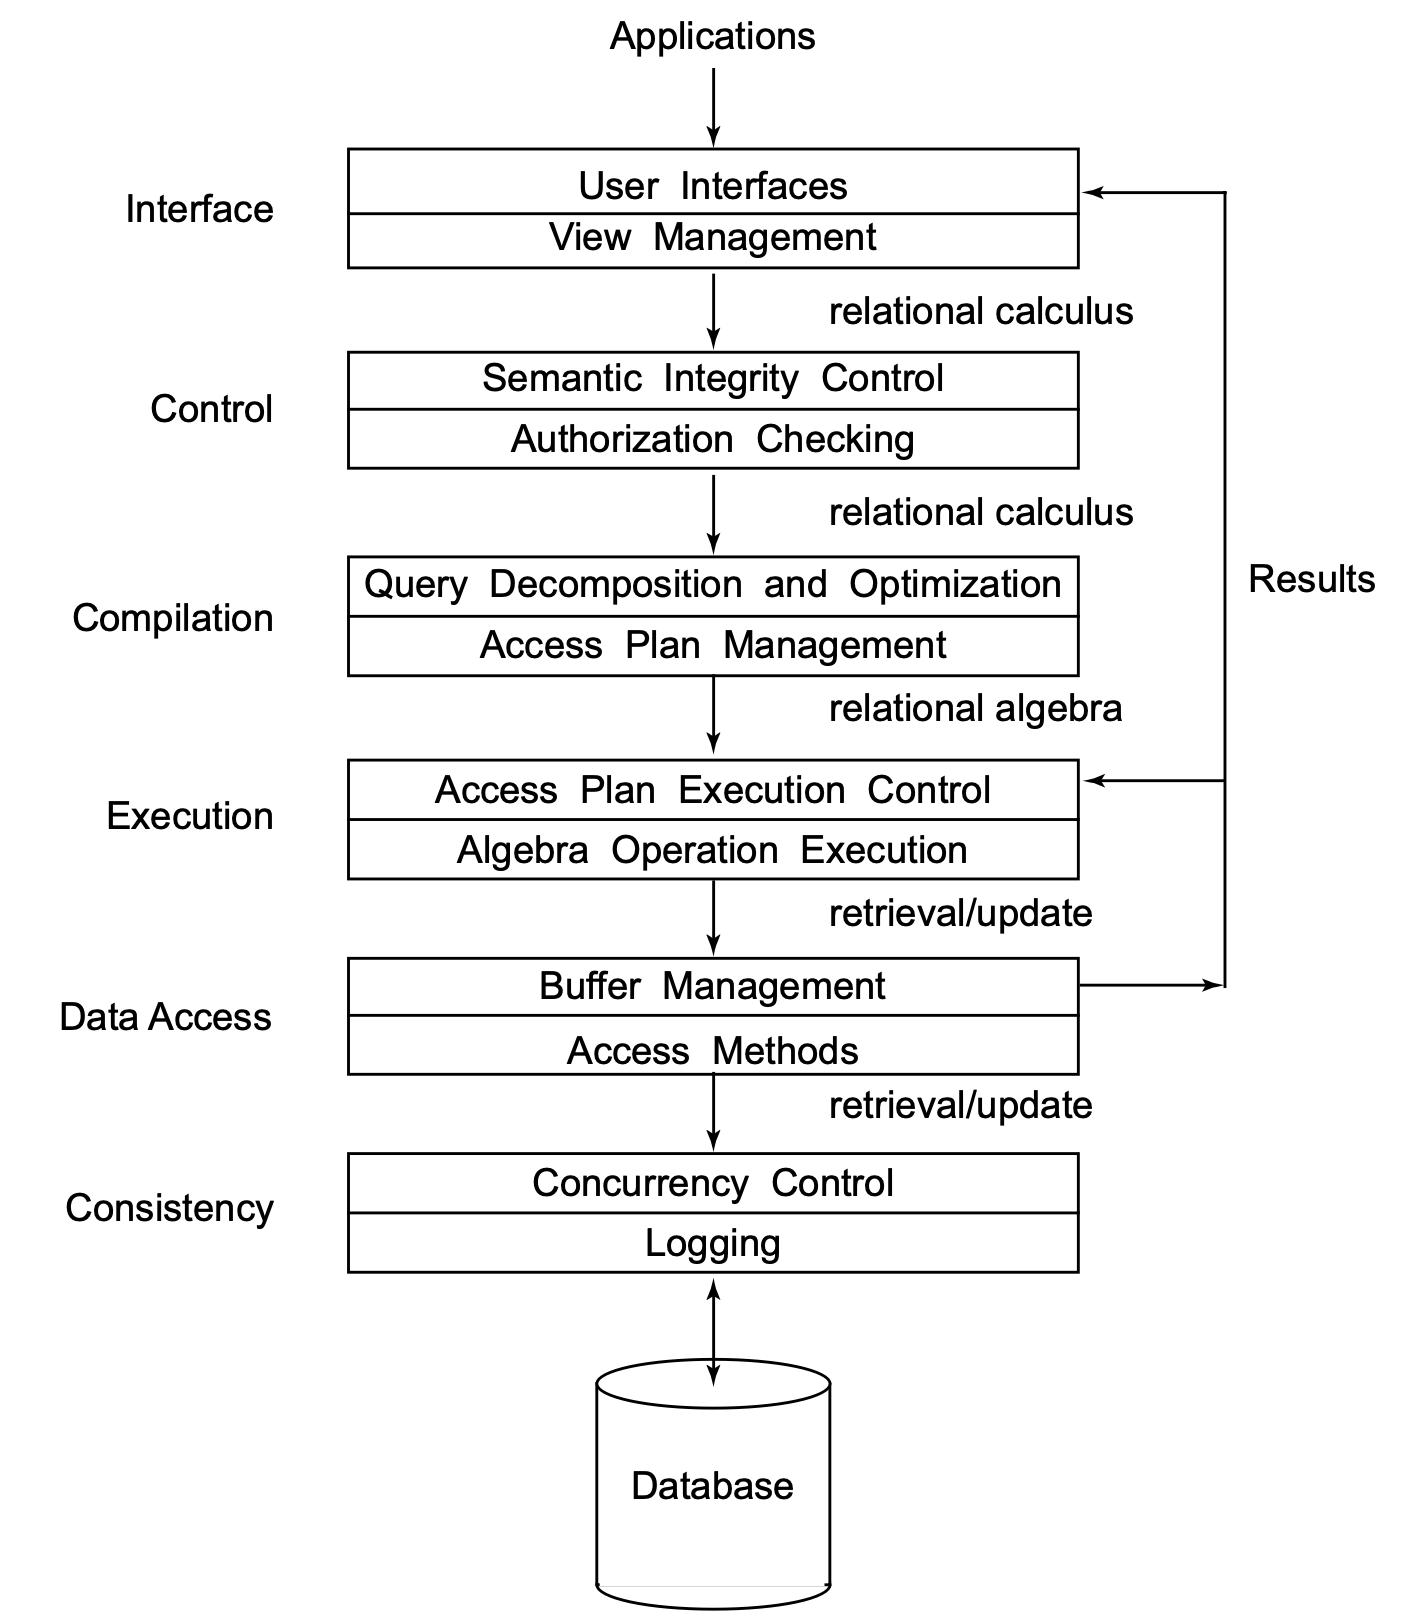
\includegraphics[width=\textwidth]{assets/functional-layers-of-centralized-dbms.png}

\subsection{Architectural Models for Distributed DBMSs}

\subsection{Autonomy}

Autonomy refers to the distribution (or decentralization) of control. The autonomy of a DBMS can span from \textit{tight integration} to \textit{semiautonomous} to \textit{total isolation}.

\subsection{Distribution}

Distribution is split into two classes: \textit{client-server} distribution and \textit{peer-to-peer} distribution (also called \textit{fully distributed}).

\subsection{Heterogeneity}

Can be found in hardware, networking protocols and data management.

\subsection{Architectural Alternatives}

\subsection{Client/Server Systems}

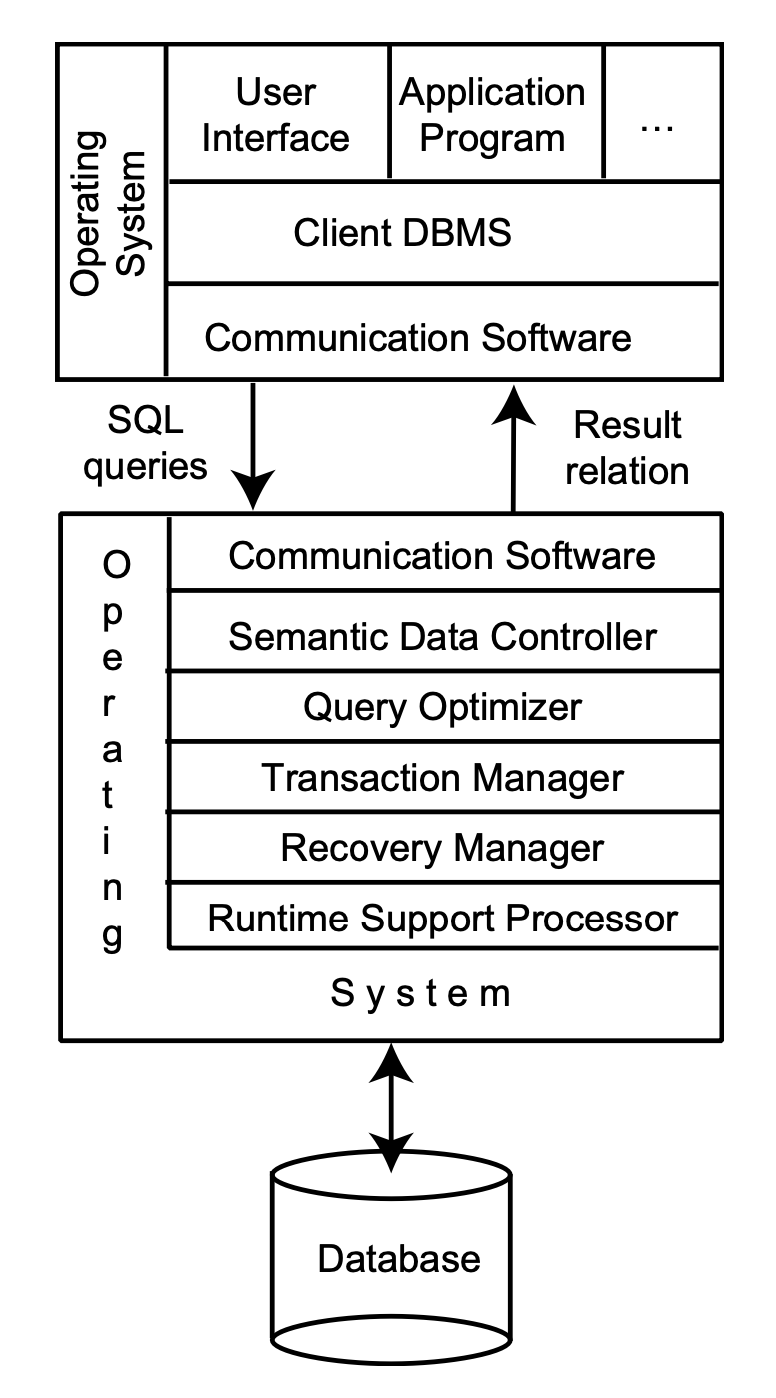
\includegraphics[scale=0.5, center]{assets/client-server-architecture.png}	

In the \textit{multiple servers}/\textit{multiple clients} approach, clients can either intentionally connect to the relevant server (\textit{heavy clients}) or connect to a "home server" which then communicates with other servers as required (\textit{light clients}).

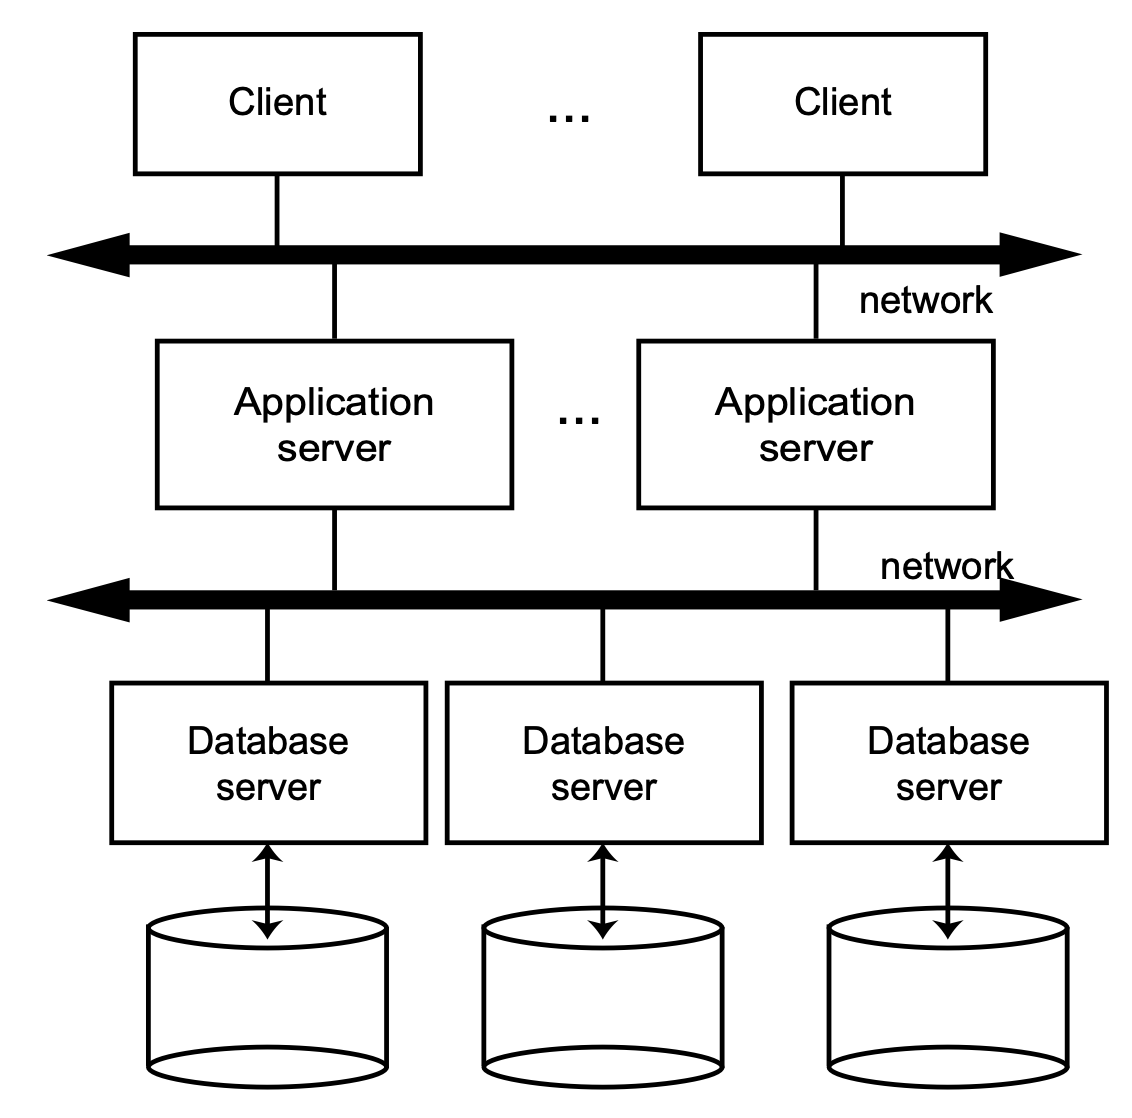
\includegraphics[scale=0.5, center]{assets/distributed-client-server-overview.png}

This is what a distributed client/server architecture would look like in the traditional three-tiered web setting.

\subsection{Peer-to-Peer Systems}

In peer-to-peer systems, there is generally no differentiation between the functionality of each site in the system.

Each site is organised in two parts within the same machine: the \textit{user processor} and \textit{data processor}. Here is an overview of the components that make up each part.

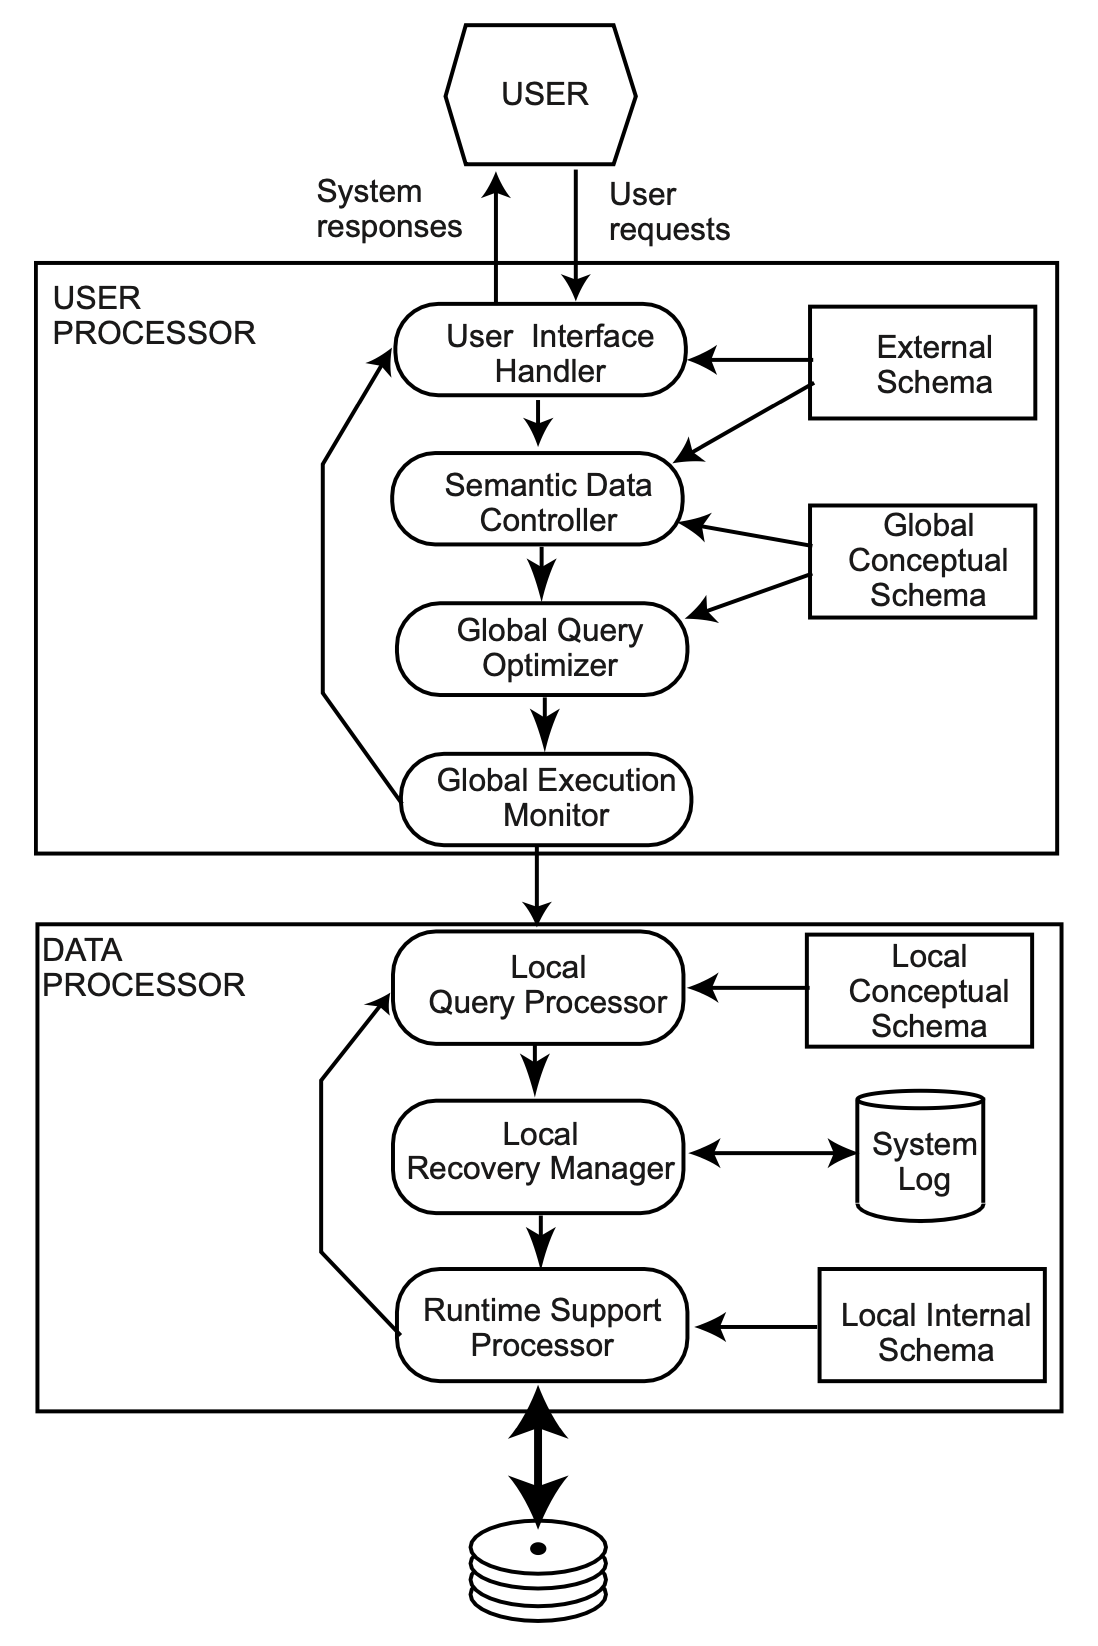
\includegraphics[scale=0.5, center]{assets/peer-to-peer-architecture.png}

\subsection{Multidatabase System Architecture}

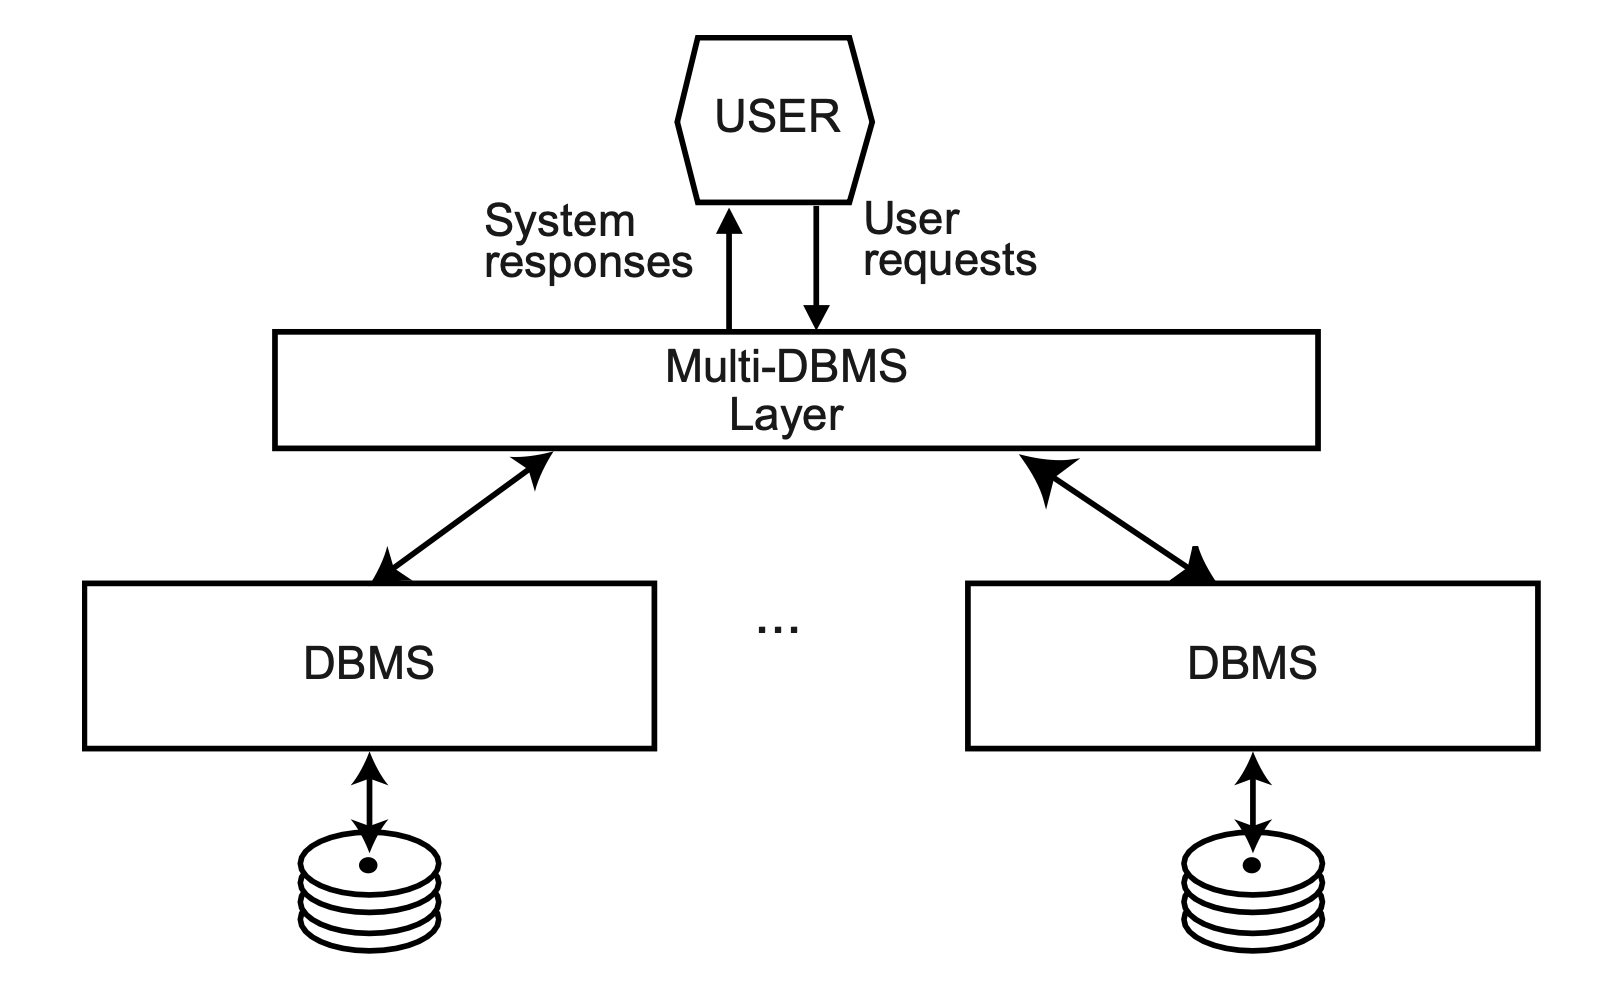
\includegraphics[scale=0.5,center]{assets/components-of-a-mdbs.png}

\end{document}
